\section{Pentaho Data Integration}
Nas seções anteriores discutiu-se um pouco sobre as principais características de um Data Warehouse e do processo CRISP-DM. Nessa seção, será discutida o uso do \pdi (PDI) no processo de ETL, como ela pode ser aplicada e suas principais características.
O PDI, também conhecido como Kettle, oferece diversas ferramentas para a extração de dados de fontes diversas, transformações, limpezas e de carregamento dos dados
\subsubsection{Arquitetura}
O \pdi é composto basicamente de quatro componentes:
\begin{itemize}
    \item Spoon: é uma aplicação \textit{desktop} de interface gráfica para a criação de \textit{jobs} e \textit{transformations}. Permite a criação de processos de ETL sem a necessidade de programação;
    \item Pan: uma interface de linha de comando que pode ser usada para a execução de \textit{transformations} e \textit{jobs} criados no \textit{spoon};
    \item Kitchen: interface de linha de comando que pode ser usada para a execução de \textit{jobs};
    \item Carte: uma aplicação \textit{web} que é capaz usar um servidor de ETL remoto, fornecendo capacidades de execução remota similares ao servidor de \textit{Data Integration}.
\end{itemize}

\subsubsection{Princípios de Design}
\citeAuthorPageYear{kettle} afirmam que o Pentaho foi desenvolvido com alguns princípios de design fundamentais. Algumas experiências negativas levaram a essas decisões. são eles:

Ele é de fácil desenvolvimento, não é preciso se preocupar com instalação de \textit{software}. Conforme \citeAuthorPageYear{kettle}, várias ferramentas baseadas em Java precisavam que o usuário especificasse explicitamente qual era o nome da Classe Java do Driver e a URL do JDBC, apenas para criar uma conexão com o banco de dados. O Kettle sempre tentou ficar longe desses problemas \citep{kettle}. Ele evita a necessidade de programar, toda linha de código adiciona complexidade e custo de manutenção ao projeto, então faz sentido não ter que lidar com isso \citep{kettle}.

O \pdi mantém as funcionalidades disponíveis na interface de usuário. \citeAuthorPageYear{kettle} afirmam que é possível realizar ETL por XML, repositório ou uma API, e todas essas opções também estão disponíveis em uma interface gráfica. Sem limitações de nomenclatura, as ferramentas de ETL precisam ser inteligentes para lidar com qualquer tipo de identificador, isso possibilita que a solução seja auto-descritiva e reduza parcialmente a necessidade de documentação \citep{kettle}.

\citeAuthorPageYear{kettle} falam que deixar que qualquer pessoa veja o que está acontecendo nas várias partes de um processo de ETL é crucial, pois oportuniza acelerar o desenvolvimento e reduzir o custo. Fluxo de dados flexível, o \pdi foi criado para ser o mais flexível possível, respeitando os fluxos que são criados \citep{kettle}. Apenas mapear dados impactados, \citeAuthorPageYear{kettle} dizem que um dos princípios fundamentais do Kettle é que todos os campos que não são mapeados passam automaticamente para o próximo passo do processo, reduzindo assim o custo de manutenção.

\subsubsection{Processo}
Ao abrir o \pdi, ele apresenta a página inicial, como mostrado na figura \ref{initialpdi}. Dessa tela é possível criar \textit{Jobs} e \textit{Transformations}, que serão explicados mais pra frente. 
\begin{figure}[H]
\centering
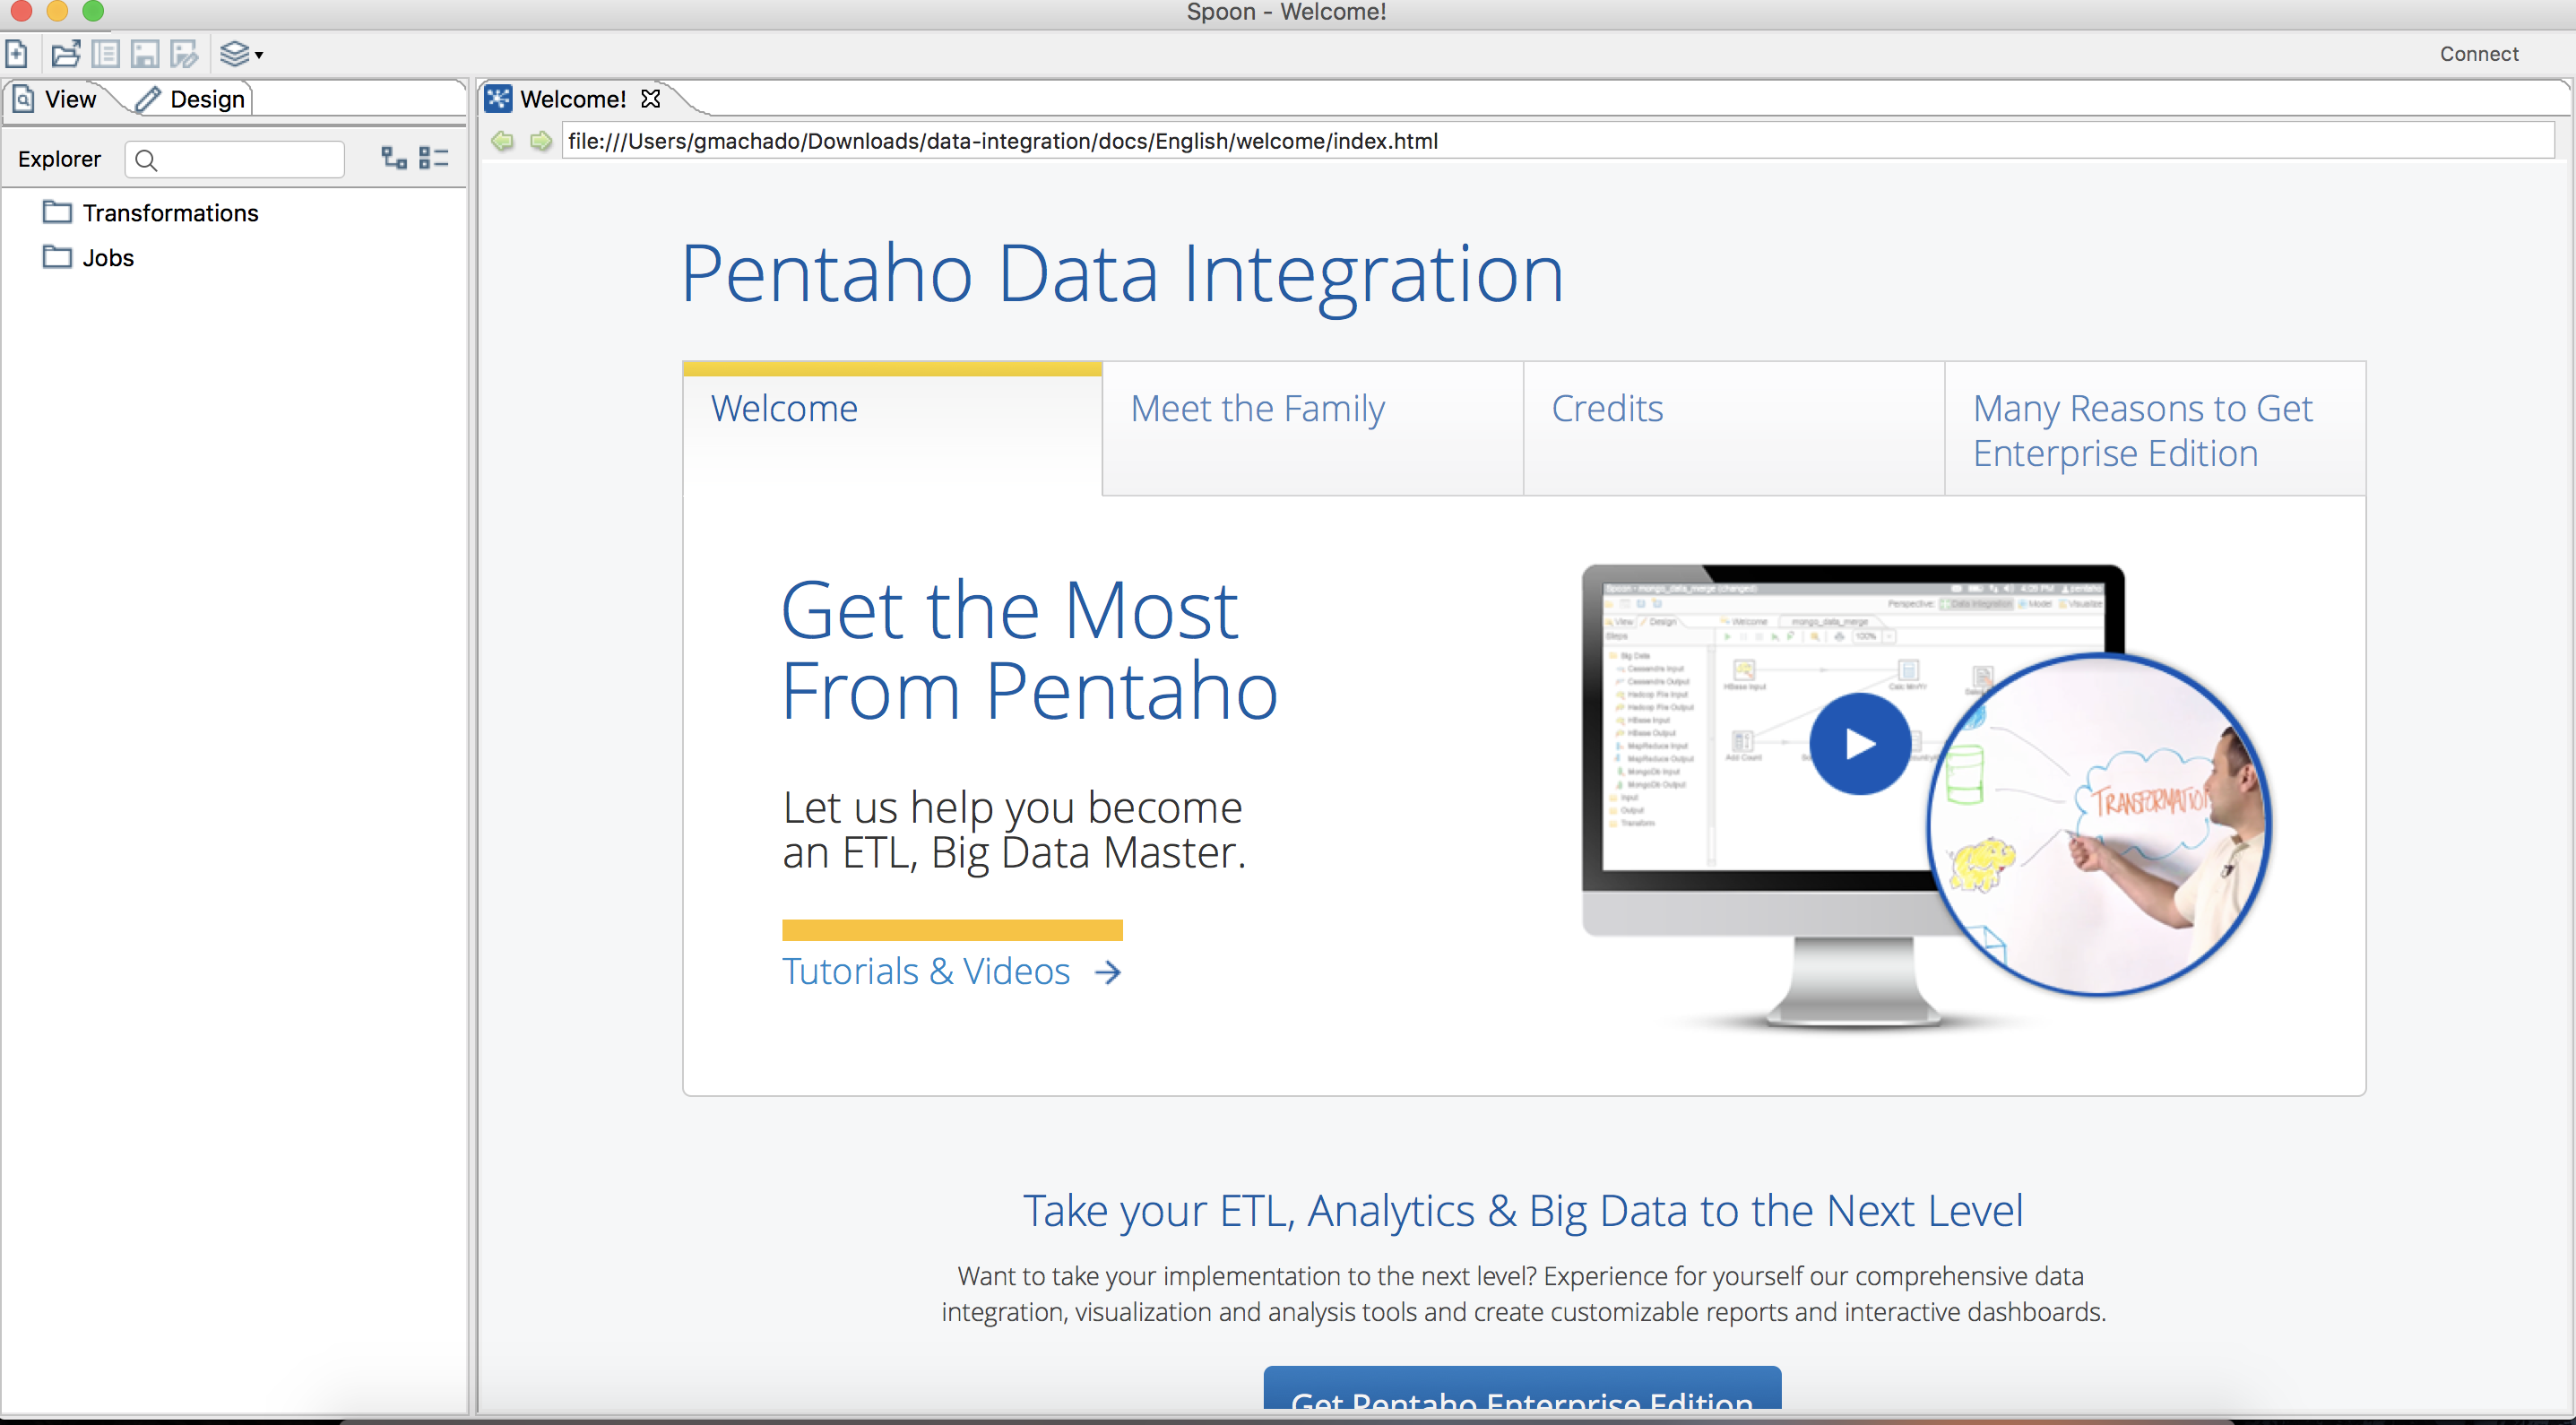
\includegraphics[height=5cm]{imagens/pagina_principal_pentaho.png}
\caption{Página inicial do \pdi}
\label{initialpdi}
\end{figure}
O \pdi tem \textit{transformations} que pode conter uma série de \textit{steps} e \textit{jobs} para realizar o processo de ETL. A figura \ref{transformationOptions} exibe algumas das opções para criação de \textit{transformations}.
\begin{figure}[H]
\centering
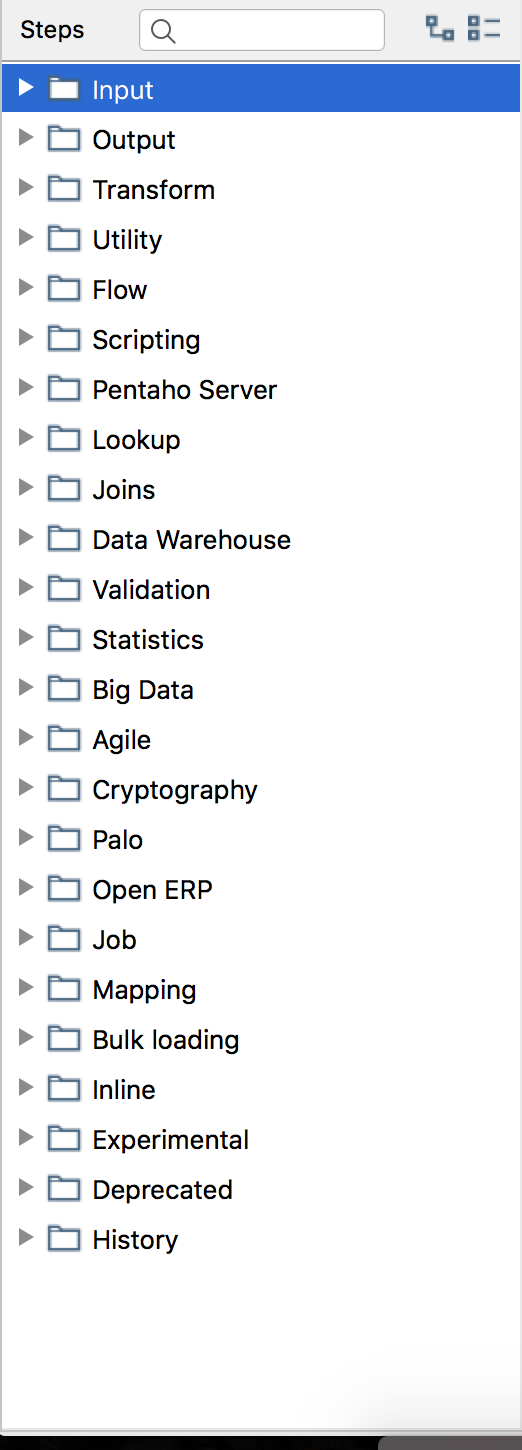
\includegraphics[width=4cm, height=8cm]{imagens/opcoes_de_transformacao.png}
\caption{Opções de transformações}
\label{transformationOptions}

\end{figure}
\textit{Transformation}, conforme \citeAuthorPageYear{kettle}, consiste em um ou mais \textit{steps}, que realizam a leitura de arquivos, filtram linhas, limpam dos dados e carregam dos dados em uma base de dados. Os \textit{steps} são conectados por \textit{hops}, que são caminhos de um único sentido por onde os dados trafegam. 

\begin{figure}[H]
\centering
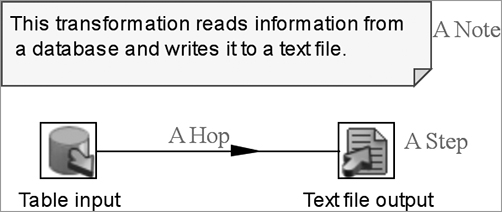
\includegraphics[height=5cm]{imagens/transformation.png}
\caption{Transformation (\citeauthor{kettle} \citeyear{kettle})}
\label{transformation}
\end{figure}

A figura \ref{transformation} mostra um pequeno exemplo de uma \textit{transformation} no \pdi.

Um \textit{step} é representado graficamente por um bloco; eles precisam ter um nome único. \citeAuthorPageYear{kettle} afirmam que um \textit{step} é capaz de ler e de escrever linhas de dados. Os \textit{steps} escrevem dados nos \textit{outcoming hops}, que são conectados a um ou mais \textit{steps} no final do \textit{hop}. Os dados são lidos nos \textit{incoming hops}. Além disso, cada \textit{step} tem uma capacidade diferente, como a figura acima mostra, na qual o primeiro irá receber dados de uma tabela e o segundo irá escrever os dados em um arquivo.

Um \textit{hop} é representado por uma seta ligando dois \textit{steps}, que define o fluxo dos dados entre eles \citep{kettle}. Um \textit{hop} também representa um \textit{buffer} de dados, chamado de \textit{row set}, que quando está cheio, o \textit{step} que escreve os dados para e quando está vazio, o \textit{step} que lê os dados aguarda até que mais dados sejam escritos.

Os \textit{jobs} são um conjunto de um ou mais \textit{jobs entries}, executados em uma certa ordem. A figura \ref{jobsOptions} exibe algumas opções que podem ser aplicadas para criar \textit{jobs}. Os\textit{ job entries}, assim como os \textit{steps}, são passos executados. Eles são conectados por meio de \textit{job hops}, que definem o caminho de execução entre os \textit{job entries} \citep{kettle}.
\begin{figure}[H]
\centering
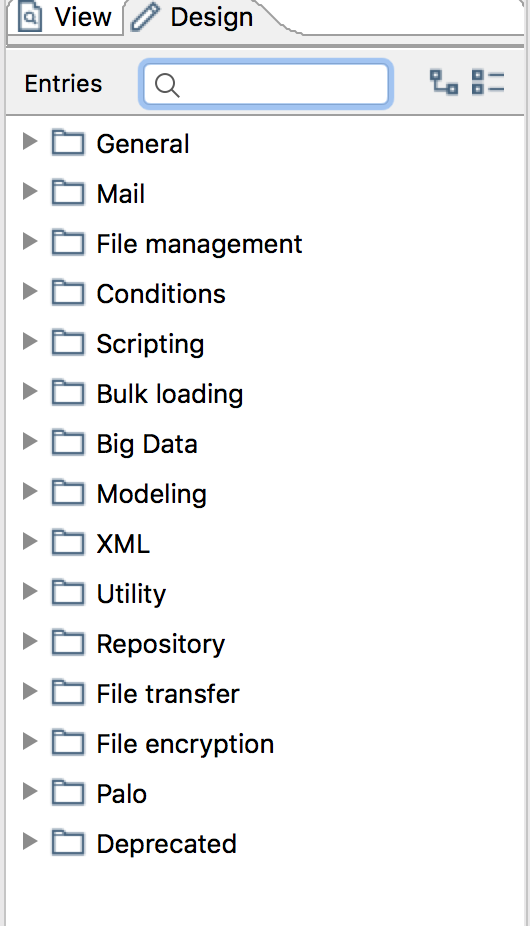
\includegraphics[width=7cm, height=9cm]{imagens/opcoes_de_jobs.png}
\caption{Opções de Jobs}
\label{jobsOptions}
\end{figure}
\subsubsection{Extract}
O \pdi oferece ferramentas para a extração dos dados de fontes como arquivos de texto, planilhas, metadados, xml, banco de dados. Como mostrado na figura \ref{inputOptions}, a opção \textit{input} tem várias ferramentas para realizar a tarefa de entrada de dados. \\
\begin{figure}[H]
\centering
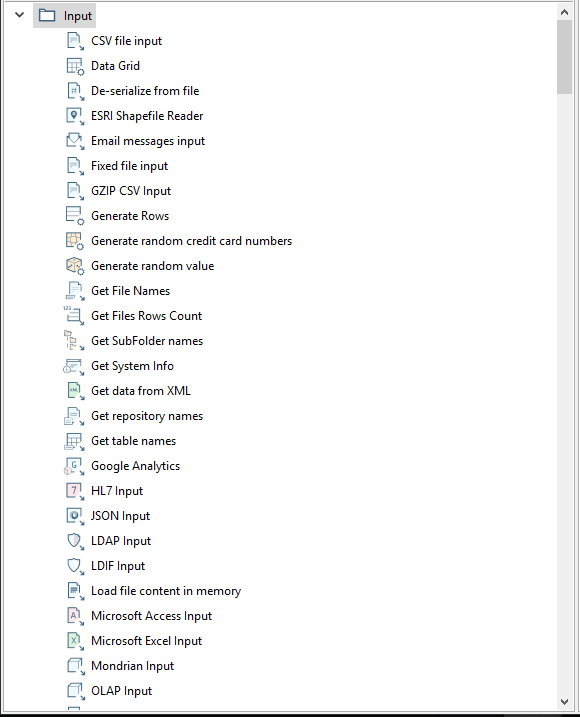
\includegraphics[width=7cm, height=9cm]{imagens/input.png}
\caption{Steps da categoria input}
\label{inputOptions}
\end{figure}
Um dos \textit{steps} responsáveis pela extração é o \textit{Text file input}, que recebe um arquivo de texto, geralmente csv, e consegue fazer a extração dos campos desejados.
No exemplo abaixo, um arquivo foi carregado com as informações da tabela \ref{autores}:\\
\begin{table}[H]
\centering
\caption{ Autores }
\vspace{0.2in}
\newcolumntype{C}{>{\centering\arraybackslash}X}%
\newcommand{\rowstyle}[1]{%
  \protected\gdef\currentrowstyle{#1}%
}
\begin{tabularx}{\textwidth}{C|C|C|C|C}
\hline 
\textbf {Sobrenome} & \textbf{Nome} &\textbf{ País } & \textbf{Ano de Nascimento} &\textbf{Ano de Falecimento} \\ \hline \hline
Machado &Gabriel &Americano &1986 &2015 \\ \hline
King &Stephen &Americano &1989 &2016 \\ \hline                         
Carlos &Matheus &Brasileiro &1988 &2016 \\ \hline                       
Maria &Ana &Americana &1980 &2009 \\ \hline                         
\end{tabularx}
\label{autores}
\end{table}
Utilizou-se um \textit{step} chamado \textit{Dummy} (figura \ref{dummy}), que não faz nada além de receber os dados:
\begin{figure}[H]
\centering
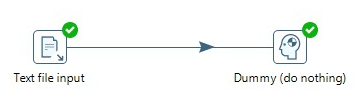
\includegraphics[height=4cm]{imagens/example1.png}
\caption{Dummy}
\label{dummy}
\end{figure}
Após a execução, as métricas de cada \textit{step} ficam disponíveis, na figura \ref{metrics} é visto que o \textit{step} \textit{"Text file input" }escreveu 5 registros e o \textit{Dummy} leu 5.
\begin{figure}[H]
\centering
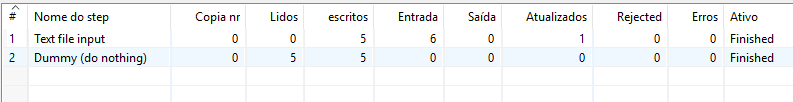
\includegraphics[height=2cm]{imagens/metrics.png}
\caption{Métricas dos steps}
\label{metrics}
\end{figure}
\vfill
\subsubsection{Transform}
Existem diversas possíveis transformações a serem aplicadas nos dados extraídos, como limpeza de campos nulos, geração de novos atributos, formatação de campos. Para isso, o \pdi oferece diversas ferramentas para realizar esse trabalho, como visto a figura \ref{transformsteps} abaixo.
\begin{figure}[H]
\centering
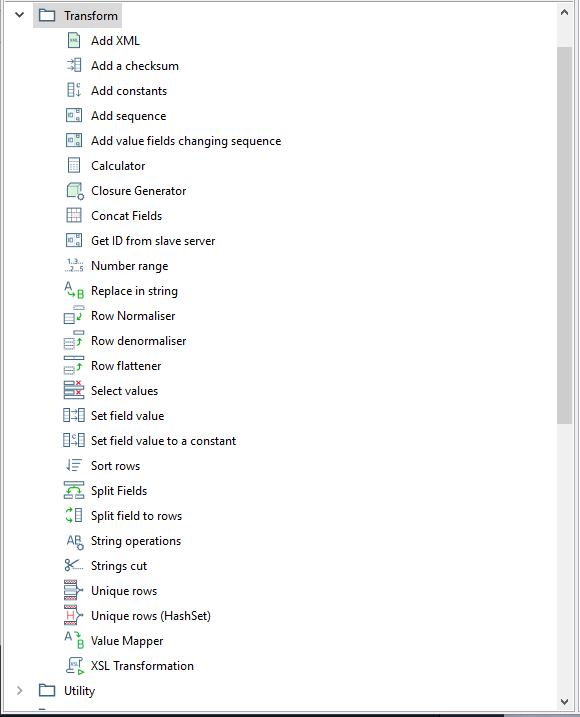
\includegraphics[width=7cm, height=9cm]{imagens/transforms.png}
\caption{Steps da categoria transform}
\label{transformsteps}
\end{figure}
Usando os mesmos dados da tabela anterior, existe a opção, como tempo de vida. Para isso um \textit{step} da aba \textit{transformation} é adicionado, o \textit{calculator} (\ref{calculator}):
\begin{figure}[H]
\centering
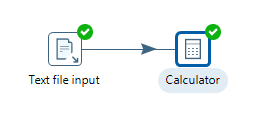
\includegraphics[height=3cm]{imagens/calc.png}
\caption{Step calculator}
\label{calculator}
\end{figure}
Esse \textit{step} irá calcular o tempo de vida da pessoa se baseando o ano de nascimento e o ano de falecimento, como mostrado na figura \ref{timespan} abaixo:
\begin{figure}[H]
\centering
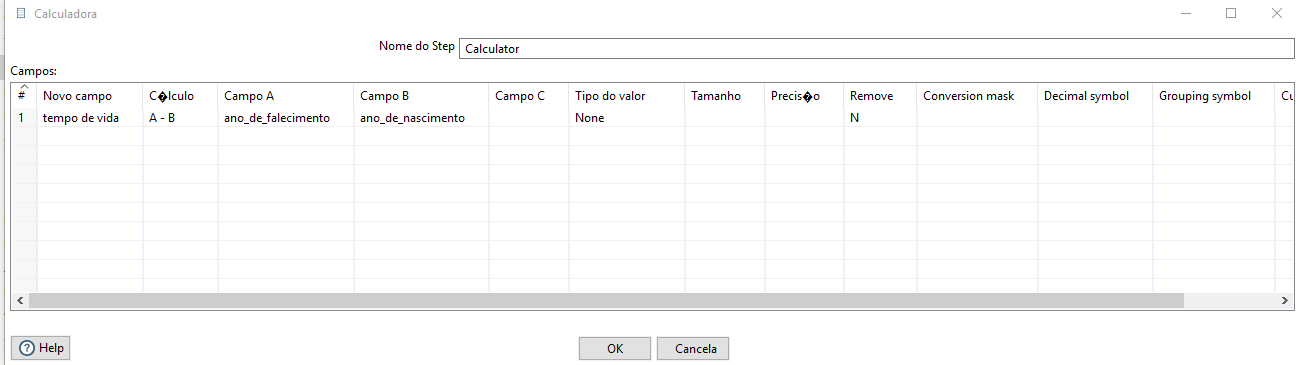
\includegraphics[height=4cm]{imagens/tempovida.png}
\caption{Cálculo do tempo de vida}
\label{timespan}
\end{figure}
A saída desse \textit{step} é ser vista no \textit{preview} (figura \ref{preview}):
\begin{figure}[H]
\centering
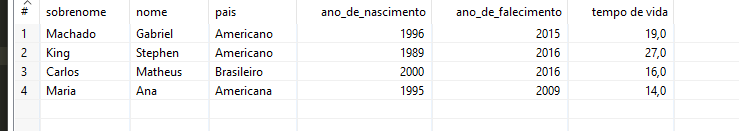
\includegraphics[height=2cm]{imagens/saidavida.png}
\caption{Saída do step}
\label{preview}
\end{figure}
\subsubsection{Load}
A última etapa do ETL é o \textit{Load} (carregamento), o \pdi oferece diversas formas de carregamento (figura \ref{outputsteps}).
\begin{figure}[H]
\centering
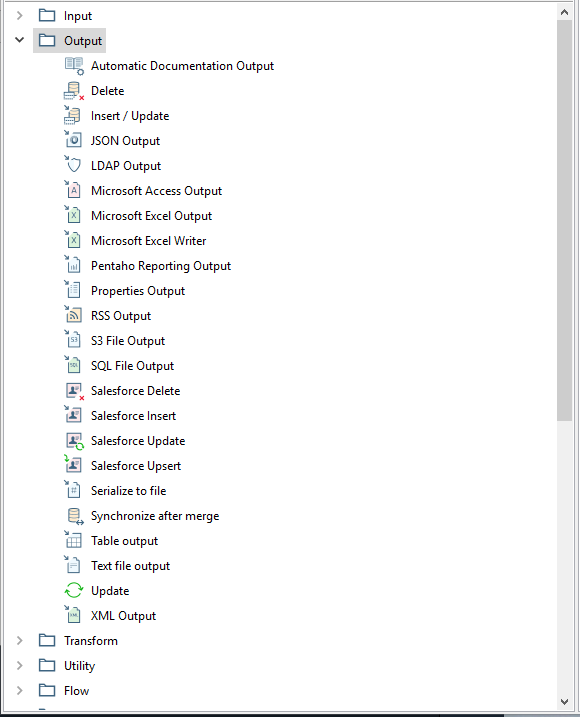
\includegraphics[width=7cm, height=9cm]{imagens/output.png}
\caption{Steps da categoria output}
\label{outputsteps}
\end{figure}
Usando os dados gerados na etapa de transformação, os dados serão carregados em uma tabela no banco de dados, para isso uma conexão no Pentaho é definida e o \textit{step} \textit{"Table output"} é criado, como mostrado na figura \ref{outputstep} abaixo.
\begin{figure}[H]
\centering
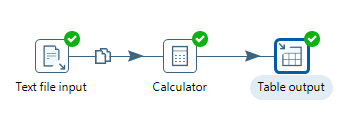
\includegraphics[height=2cm]{imagens/tableoutput.png}
\caption{Saída no banco de dados}
\label{outputstep}
\end{figure}
Na aba \textit{view}, na figura \ref{database}, existe uma opção \textit{connections} e lá tem como criar uma conexão com a base de dados escolhida, nesse caso é o postgres.\\
\begin{figure}[H]
\centering
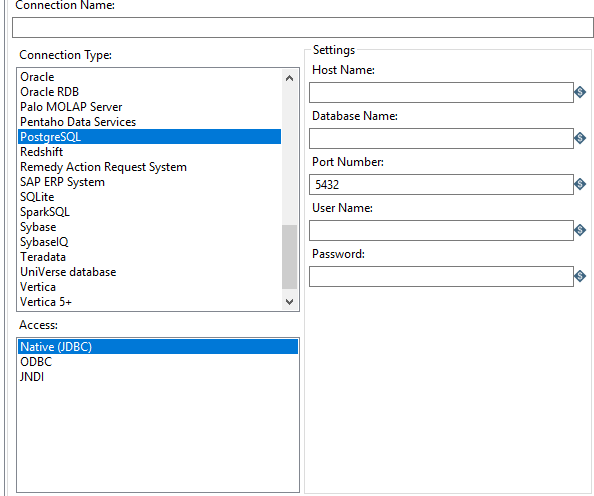
\includegraphics[height=7cm]{imagens/conexao.png}
\caption{Conexões disponíveis no \pdi}
\label{database}
\end{figure}
Quando a conexão for definida, o step \textit{table output }(figura \ref{outputtable}) é criado, realizando o mapeamento adequado dos campos para serem inseridos na tabela.
\begin{figure}[H]
\centering
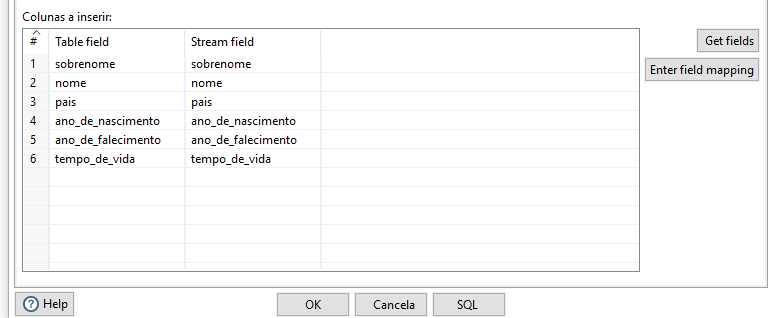
\includegraphics[height=3cm]{imagens/tablemapping.png}
\caption{Mapeamento entre os campos gerados e os campos da tabela}
\label{outputtable}
\end{figure}
Ao executar a transformação, os dados serão carregados na tabela, como mostra a figura \ref{table}.
\begin{figure}[H]
\centering
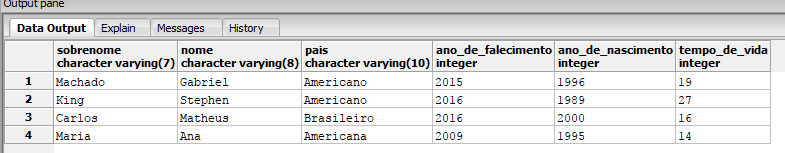
\includegraphics[height=2.5cm]{imagens/saidasql.png}
\caption{Saída no banco de dados}
\label{table}
\end{figure}

\section{Mineração de Dados}

O termo mineração de dados poderia ter sido chamado de mineração de conhecimentos dos dados \citep{jmj}, já que minerar é um processo para encontrar pequenas quantidades de preciosidades de uma grande quantidade de material bruto. 

Outros dizem que mineração de dados é um sinônimo de KDD (\textit{knowledge discovery from data}), descobrimento de conhecimento a partir de dados. A mineração também é vista como um passo essencial no processo de descoberta de conhecimento, como mostra a figura \ref{kdd}. 

\begin{figure}[H]
\centering
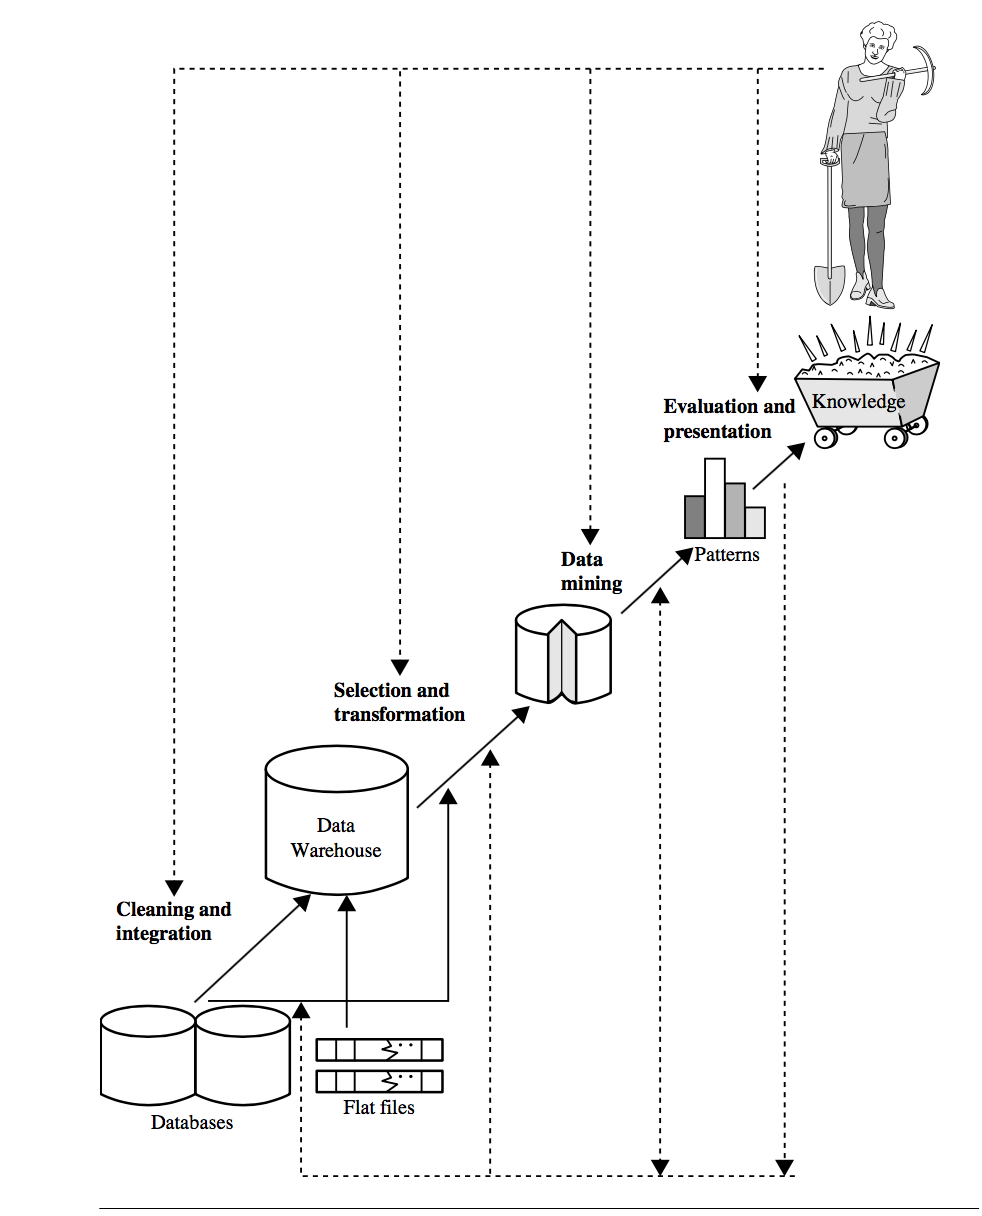
\includegraphics[height=9cm, width=9cm]{imagens/kdd.png}
\caption{Mineração de dados como um processo de descoberta de conhecimento \citep{jmj}}
\label{kdd}
\end{figure}

\citeauthor{jmj} sumarizam mineração de dados como o processo de descobrir padrões interessantes e conhecimento a partir de grandes quantidades de dados. Essas fontes podem ser banco de dados, a internet, \textit{data warehouses}, dados transacionais, \textit{stream} de dados, arquivos etc. 

A mineração de dados tem diversas funcionalidades, como caracterização (sumarização das características gerais de uma classe alvo de dados) e discriminação (comparação das características gerais de uma classe alvo com as características de uma ou mais classes diferentes) \citep{jmj}. 

Também é usada para encontrar padrões que aparecem frequentemente nos dados. Existem alguns tipos de padrões, como \textit{frequent itemset}, itens que geralmente aparecem juntos em um conjunto de dados transacionais, \textit{frequent subsequence} ou \textit{sequencial pattern}, que, por exemplo, é o padrão de um cliente que compra primeiro um \textit{notebook}, seguido de uma câmera digital e então um cartão de memória \citep{jmj}. Por último, tem as \textit{frequent substructures}, que são formas estruturadas que aparecem frequentemente, como grafos e árvores, que podem conter \textit{itemsets} e \textit{subsequences}  \citep{jmj}.

Algoritmos de classificação e regressão são usados para análises preditivas, tentando prever dados categóricos ou discretos. A classificação é o processo de encontrar um modelo que melhor expressa uma classe. Esse modelo é derivado da análise de um conjunto de treinamento \citep{jmj}. Os modelos são representados usando árvores de decisão, fórmulas matemáticas, redes neurais etc.

Já a regressão, o uso mais comum é para tentar prever valores numéricos contínuos, com algoritmos como regressão linear, regressão LASSO etc.

Também existem os algoritmos de clusterização, que, diferentemente da classificação e regressão, analisam os dados sem consultar as suas classes \citep{jmj}. Em alguns casos, os dados até vem sem classe. \citeauthor{jmj} dizem que a clusterização é ser usada para encontrar classes para os grupos de dados. Os \textit{clusters} são formados de uma forma que os objetos dentro deles tenham uma grande similaridade ao se compararem uns com os outros, mas se diferenciam dos objetos em outros \textit{clusters} \citep{jmj}.

\subsection{CRISP-DM}
\subsubsection{O que é CRISP-DM}
CRISP-DM, ou\textit{ Cross-industry standard process for data mining}, é uma técnica aplicada no processo de mineração de dados, com uma série de tarefas a serem realizadas para chegar ao melhor resultado.
Segundo \citeAuthorPageYear{dmfd}, a mineração de dados não é algo feito uma vez e depois esquecido, o trabalho pode ser aplicado em outros projetos, servir de referência.
O ciclo de vida da mineração de dados contém seis fases, como apresentado na figura \ref{crispcycle}: entendimento do negócio, entendimento dos dados, preparação dos dados, modelagem, avaliação e implementação. 
A mineração de dados não termina uma vez que a solução é implementada \citep{crispmanual}
\begin{figure}[H]
\centering
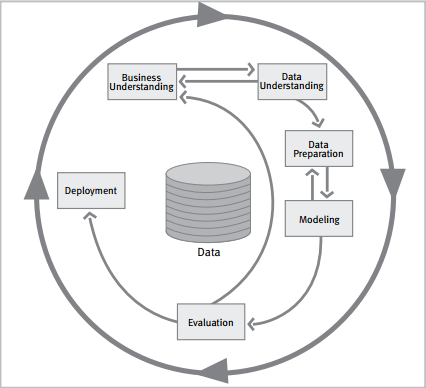
\includegraphics[height=6.2cm]{imagens/lifecycle.png}
\caption{Ciclo de vida (\citeauthor{crispmanual} \citeyear{crispmanual})}
\label{crispcycle}
\end{figure}
As fases tem diversas tarefas que são realizadas para completa-las e toda tarefa tem suas saídas.
\subsubsection{Entendimento do negócio}
A primeira etapa do CRISP-DM é o entendimento do negócio, que foca em esclarecer os objetivos do negócio e seus requerimentos de uma perspectiva de negócio.

O primeiro objetivo da análise de dados é entender, sob uma perspectiva de negócio, o que o cliente deseja realizar. Segundo \citeAuthorPageYear{dmfd}, deve-se ter um entendimento claro do problema que se deseja abordar, o objetivo do negócio, as limitações e o impacto. Esse processo produz uma informação da situação do negócio, objetivo do cliente e o critério de sucesso.

Em seguida é realizada uma avaliação da situação. Essa tarefa consiste em um detalhamento maior dos recursos, limitações, premissas e outros fatores que devem ser considerados ao determinar os objetivos da análise de dados e do plano de projeto \citep{crispmanual}.

Outra etapa é determinar os objetivos da mineração de dados, por exemplo, como "prever quantas pessoas irão visitar uma loja no verão, de acordo com informações dos últimos 2 anos dessa loja".

E então produzir plano de projeto, ou seja, o plano desejado para atingir os objetivos da mineração de dados e desse modo, os objetivos do negócio \citep{crispmanual}. Esse processo produz o plano de projeto e avaliações iniciais de ferramentas e técnicas.

\subsubsection{Entendimento dos dados}
De acordo com \citeAuthorPageYear{dmfd}, na segunda etapa do projeto de mineração de dados, os dados têm que ser obtidos e deve-se verificar se eles são apropriados para as necessidades.

A primeira tarefa desse processo é coletar dados iniciais e então realizar, caso necessário, o carregamento dos dados em alguma ferramenta. Nessa tarefa é produzida uma lista de todos os \textit{datasets} adquiridos, junto com localizações, métodos realizados para coleta e problemas encontrados.

A próxima tarefa é descrever os dados dos dados, explora-se eles usando técnicas de visualização. Essa análise esta diretamente ligada aos objetivos da mineração de dados \citep{crispmanual}. Essa tarefa produz um relatório da exploração de dados, contendo descobertas iniciais ou hipóteses, e o seu impacto no restante do projeto \citep{crispmanual}.

Depois, é necessário verificar a qualidade dos dados, respondendo perguntas como "os dados estão completos?", "existem valores faltantes?". É criado um relatório da qualidade dos dados, com uma lista de problemas encontrados e suas soluções.

\subsubsection{Preparação dos Dados}
A maior parte do tempo gasto no processo de mineração de dados é na preparação deles, já que diversos tratamentos precisam ser feitos nos dados e isso nem sempre é tão simples. A maior parte dos dados usados para mineração foi originalmente coletada e preservada para outros objetivos e precisa ser refinada antes de ser ficar pronta para a modelagem \citep{dmfd}.

Essa parte tem duas saídas, antes das tarefas, que são: \textbf{datasets}, dados produzidos e que serão usados para modelagem e \textbf{descrição do dataset} \citep{crispmanual}.

A primeira tarefa é \textbf{selecionar os dados} que serão usados na modelagem, baseando-se nos objetivos da mineração de dados, qualidade e limites técnicos \citep{crispmanual}. É criada uma lista de dados que foram incluídos e excluídos e a razão para isso.

Posteriormente é feita uma \textbf{limpeza dos dados}, que eleva a qualidade dos dados para o nível requerido pelas técnicas de análise selecionadas \citep{crispmanual}. De acordo com \citeAuthorPageYear{dmfd}, dificilmente os dados selecionados estarão perfeitamente limpos, mudanças precisarão ser feitas nos dados para atingir o nível necessário. \citeAuthorPageYear{crispmanual} falam que transformações nos dados são feitas para limpeza e possível impacto na análise de resultados. Nessa etapa é criado um relatório de limpeza de dados: que descreve as ações tomadas para lidar com os problemas encontrados anteriormente.

A tarefa seguinte é \textbf{Construir dados}, que consiste na criação de novos campos, dados agregados, ou novos formatos de dados. É produzida uma lista de atributos derivados a partir dos que já existem e explica como e por que eles foram gerados e uma lista de registros criados, junto com o motivo e como eles foram formados.

A próxima tarefa é \textbf{integrar dados}, já que existe a possibilidade deles estarem em diferentes \textit{datasets} e é necessário a integração desses dados para a próxima etapa, modelagem. A saída desse passo é: \textbf{dados fundidos}: fundir tabelas se refere a juntar duas ou mais tabelas que têm diferentes informações sobre o mesmo objeto \citep{crispmanual}. 

Por último, a tarefa \textbf{formatar dados} é aplicada. Dados frequentemente vêm em formatos que não são os convencionais para modelagem \citep{dmfd}, então conversões precisam ser feitas. \citeAuthorPageYear{dmfd} afirma que o processo de preparação de dados deve ser finalizada com um \textit{dataset} pronto para modelagem e um relatório descrevendo o \textit{dataset}.

A saída é dados reformatados, convertidos para alguma unidade de medida única para todos os dados (como quilos, em peso).

\subsubsection{Modelagem}
É a etapa na qual alguma técnica de aprendizado de máquina é aplicada, testada e avaliada para encontrar padrões nos dados, como \textit{K-nearest neighbors}, \textit{Decision Tree }e etc.

O primeiro passo da modelagem é \textbf{selecionar a técnica de modelagem} que será usada. Caso múltiplas técnicas sejam aplicadas, é preciso executar essa tarefa para cada uma delas \citep{crispmanual}. Nem todas as técnicas de modelagem serão úteis para as necessidades do negócio.

Em seguida, o \textbf{teste de design} é gerado, ou seja, procedimentos ou mecanismos para testar a qualidade e validade do modelo \citep{crispmanual}. Os dados geralmente são separados em dois conjuntos, o de treinamento e o de teste. O de treinamento é usado para construir o modelo e o de teste para validar ele. Nessa etapa é gerado descrito como planeja, treina, testa e avalia o modelo.

Depois, é o momento de \textbf{construir o modelo}, rodar a ferramenta de modelagem para criar um ou mais modelos \citep{crispmanual}. Esse processo produz um documento com as configurações de parâmetros usados, modelos produzidos pela ferramenta e uma descrição deles.

Por fim, é a fase de \textbf{avaliar o modelo}, que sumariza os dados e ranqueia os modelos e também revisa as configurações dos parâmetros aplicados para tentar reajustá-los até encontrar a melhor possível.

\subsubsection{Avaliação}
Avaliar todo o processo: não só os modelos, mas também o processo empregado para a sua criação.

A primeira tarefa é \textbf{avaliar resultados}. Ela avalia o grau em que o modelo se adequa ao objetivo original do negócio e busca determinar se existe alguma razão para o modelo estar deficiente.

Ela também avalia o resultado da mineração de dados a respeito do critério de sucesso do negócio, \citeAuthorPageYear{dmfd} mostra que esse processo serve para dizer se o projeto atingiu ou não os objetivos definidos no início e seleciona os modelos que atingiram o critério selecionado.

Após a última tarefa, é feita uma \textbf{revisão do processo}, nesse ponto, os modelos resultantes aparentam ser satisfatórios para a necessidade do negócio \citep{crispmanual}. Essa é um passo usado para rever o processo, como algum problema que foi negligenciado. \citeAuthorPageYear{crispmanual} mostram que se deve sumarizar a revisão e ressaltar as atividades que não foram realizadas e aquelas que devem ser repetidas.

A última fase é \textbf{determinar próximos passos}. A fase de avaliação é concluída com as recomendações para o próximo passo \citep{dmfd}. Decidir se deve finalizar o projeto ou continuar o desenvolvimento. Essa fase também inclui a análise das despesas e recursos restantes, que tem influencia na decisão \citep{crispmanual}.
Essa etapa produz uma lista de possíveis ações e a decisão.

\subsubsection{Implementação}
O objetivo dessa última parte é a implementação do modelo.
O primeiro passo é o plano de implementação, usando os resultados da avaliação e determina a estratégia de implementação \citep{crispmanual}. 

A primeira parte é gerar um plano que sumariza as estratégias para implementação, os passos necessários e como realizar.
Posteriormente é feito um \textbf{Plano de monitoramento e manutenção}, conforme \citeAuthorPageYear{dmfd} diz, a mineração de dados é um ciclo, então existe a necessidade continuar envolvida com os modelos enquanto eles são integrados ao dia-a-dia. A preparação cuidadosa das estratégias de manutenção ajuda a evitar longos períodos desnecessários de uso incorreto dos resultados da mineração \citep{crispmanual}.

Em seguida é produzido um plano de monitoramento e manutenção que sumariza todas as estratégias de manutenção e monitoramento, incluindo os passos necessários para realizá-los \citep{crispmanual}.
Em seguida, é feito um \textbf{Relatório Final}, um sumário do projeto e das experiências ou uma apresentação final e compreensível dos resultados da mineração \citep{crispmanual}.
Essa etapa produz o relatório final, que sumariza todo o projeto ao juntar todos os relatórios criados até o momento \citep{dmfd} e apresentação final, um encontro realizado na conclusão do projeto com seu cliente.

Por último, é feita uma \textbf{revisão do projeto} na qual o time se reúne e discute o que deu e não deu certo, o que pode e não pode ser feito novamente, e coisas que devem ser evitado \citep{dmfd}.
A saída é uma documentação de experiência que sumariza a experiência ganha com o projeto, como erros e acertos, dicas de como selecionar os melhores modelos para situações semelhantes etc.

\subsection{WEKA}

O WEKA, \textit{Waikato Environment for Knowledge Analysis}, é uma coleção de algoritmos de aprendizado de máquina e de ferramentas de preprocessamento de dados \citep{weka}. Ele é criado de uma forma que os algoritmos possam ser testados rapidamente nos \textit{datasets}. Também contém suporte de mineração de dados, como preparação dos dados, avaliar modelos estatisticamente, visualização dos dados e resultados da aprendizagem. Todas essas ferramentas estão disponíveis em uma interface simples. O WEKA é escrito em Java e é distribuído sob a GNU \textit{(General Public License)}, rodando em quase toda plataforma e já tendo sido testado nos sistemas operacionais Linux, Windows e Macintosh \citep{weka}.

\citeAuthorPageYear{weka} afirmam que o WEKA contém métodos para os principais problemas de mineração de dados, como regressão, clusterização, mineração de regras de associação e seleção de atributos. Conhecer os dados é uma parte integral do trabalho. Uma das formas de se usar o WEKA é aplicando um método aos dados e analisando a saída para aprender mais sobre os dados \citep{weka}, outra é selecionando modelos para gerar previsões em novas instâncias. Uma terceira forma é aplicar diferentes algoritmos e comparar as performances para então selecionar um para previsão \citeAuthorPageYear{weka}. \citeAuthorPageYear{weka} dizem que a implementação de algoritmos de aprendizado é um dos recursos mais valiosos que o WEKA fornece, enquanto os métodos de preprocessamento, também chamados de \textit{filters}, vêm logo após. 

Nas palavras de \citeAuthorPageYear{weka}, o WEKA é facilmente usado através de uma interface gráfica chamada de \textit{Explorer}. Por exemplo, um \textit{dataset} é facilmente carregado e construir uma árvore de decisão em cima dele. O WEKA também tem outras interfaces, como o \textit{Knowledge Flow}, que facilita processar dados via \textit{streaming} e o \textit{Experimenter}, que permite responder uma pergunta bem básica e prática: quais métodos e valores de parâmetros funcionam melhor para determinado problema? O WEKA fornecer um ambiente que possibilita aos usuários do WEKA comparar uma variedade de algoritmos de aprendizado. \citeAuthorPageYear{weka} ainda falam que é possível fazer isso interativamente usando a  interface \textit{Explorer}, mas o \textit{Experimenter} facilita a automatização do processo, deixando mais fácil de rodar classificadores e filtros em um \textit{dataset}, para coletar estatísticas de performance.

Além disso, todas essas opções podem ser acessadas através de uma interface de linha de comando.

\subsection{Explorer}
A interface gráfica principal do WEKA é a \textit{Explorer}. Diversas operações são feitas nessa interface.

\subsubsection{Carregando os dados}
Ao abrir o WEKA, deve-se selecionar a opção \textit{explorer}, como mostrado na figura \ref{explorer}:

\begin{figure}[H]
\centering
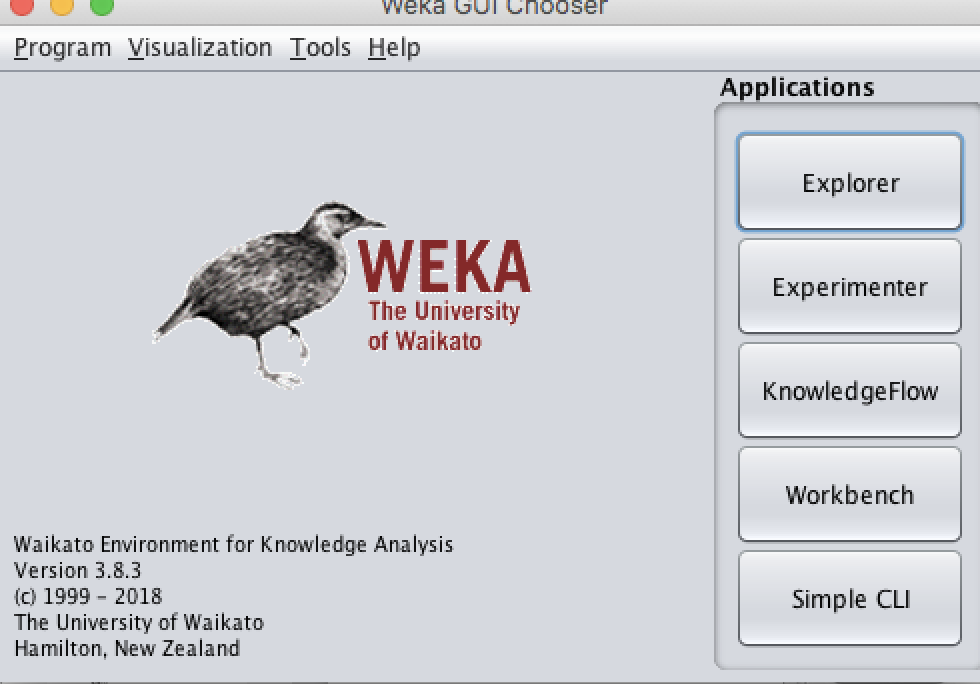
\includegraphics[height=5cm]{imagens/wekaprincipal.png}
\caption{Interface principal do WEKA}
\label{explorer}
\end{figure}

Ao abrir o \textit{explorer}, a tela deverá exibir diversas opções para carregamento de dados. O formato principal do WEKA é o ARFF, porém ele também é capaz de ler outros formatos, como csv.

\begin{figure}[H]
\centering
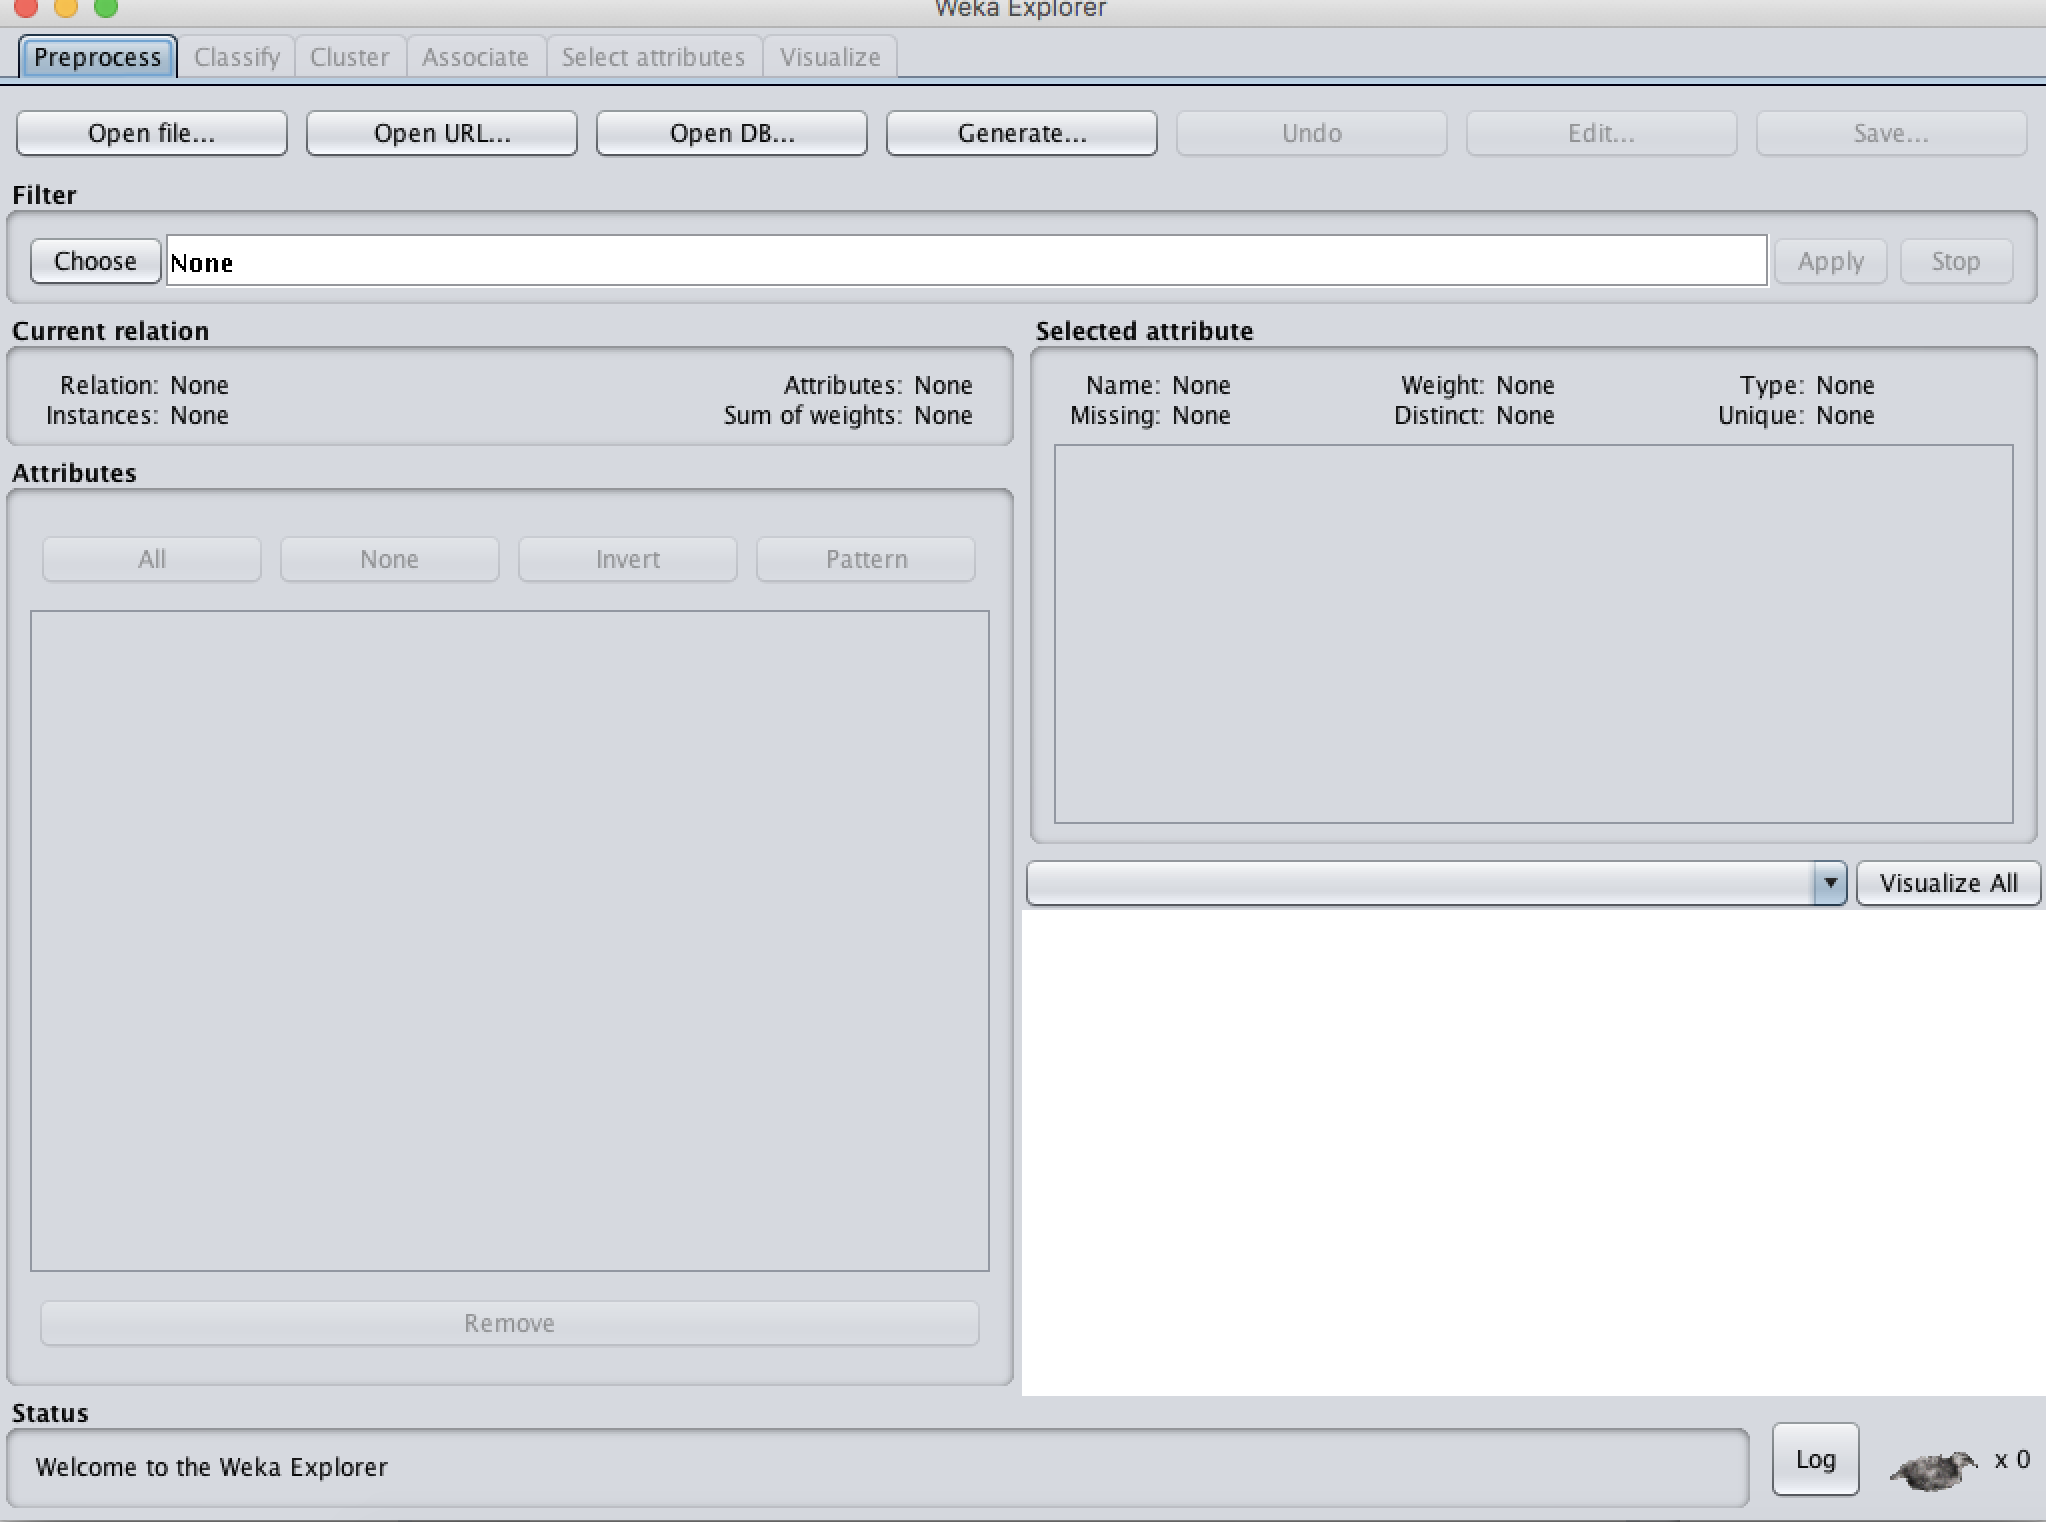
\includegraphics[height=7cm]{imagens/wekapreprocessempty.png}
\caption{Tela de preprocessamento}
\label{figura19}
\end{figure}

Ao carregar os dados, informações sobre cada um dos atributos é exibida no canto inferior direito e todos os atributos estarão listados no canto esquerdo, como visto na figura \ref{loadeddata}. A figura \ref{distribuicao} mostra que é possível obter uma distribuição dos valores de cada um dos atributos disponíveis.

\begin{figure}[H]
\centering
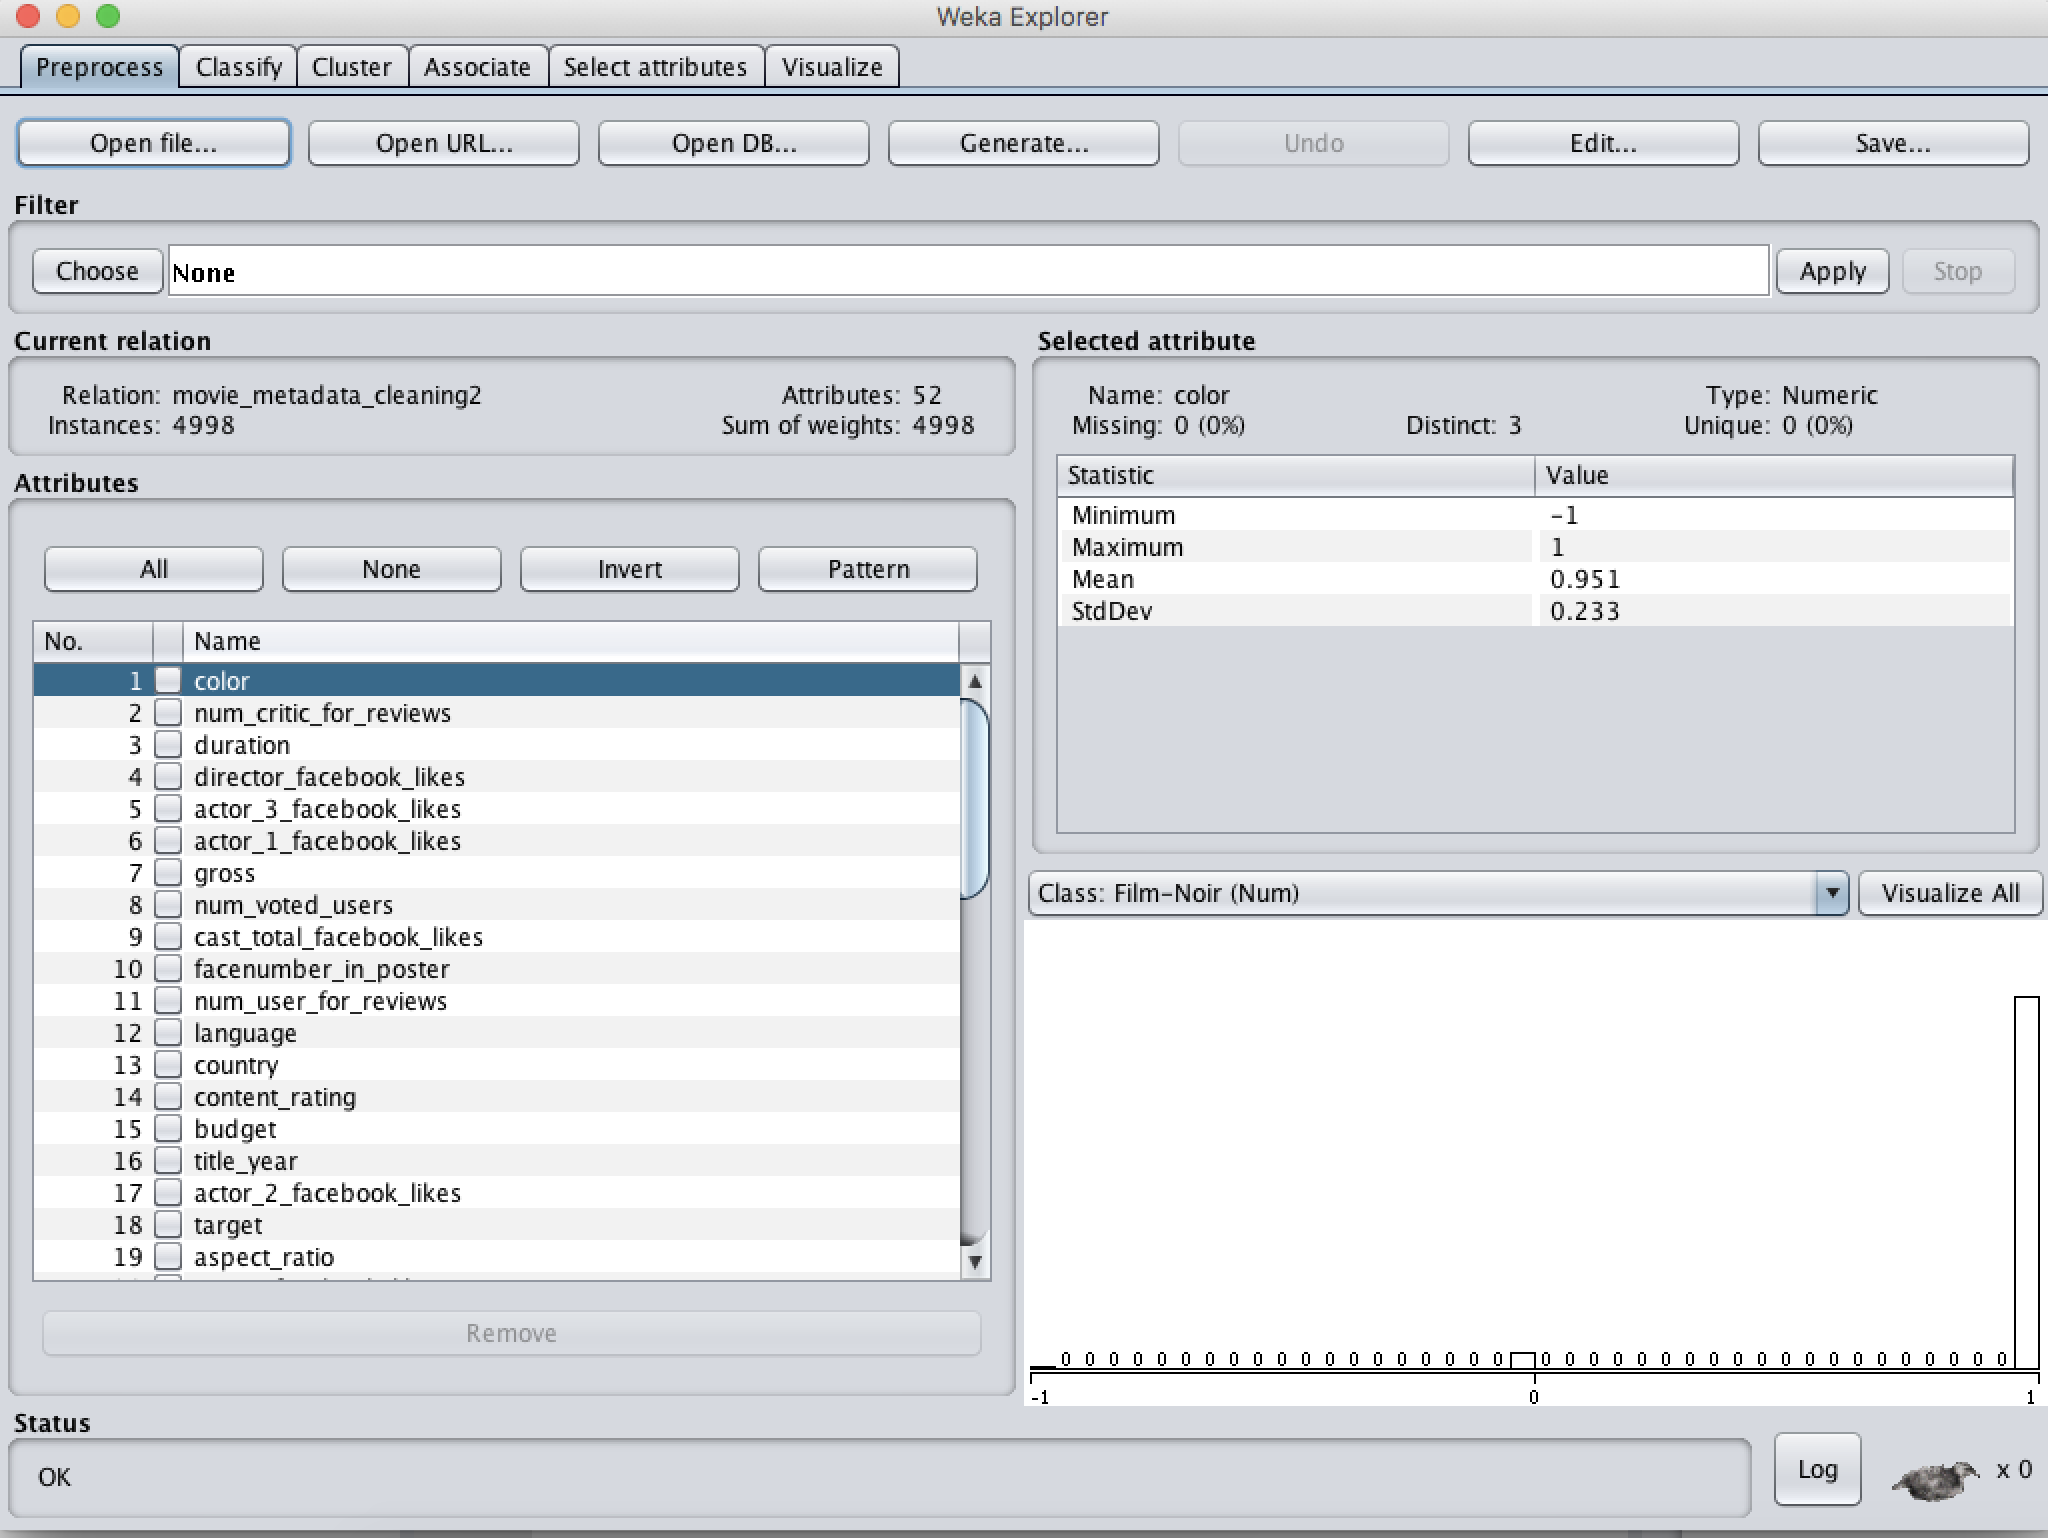
\includegraphics[height=7cm]{imagens/wekapreprocessingfull.png}
\caption{Dados carregados}
\label{loadeddata}
\end{figure}

\begin{figure}[H]
\centering
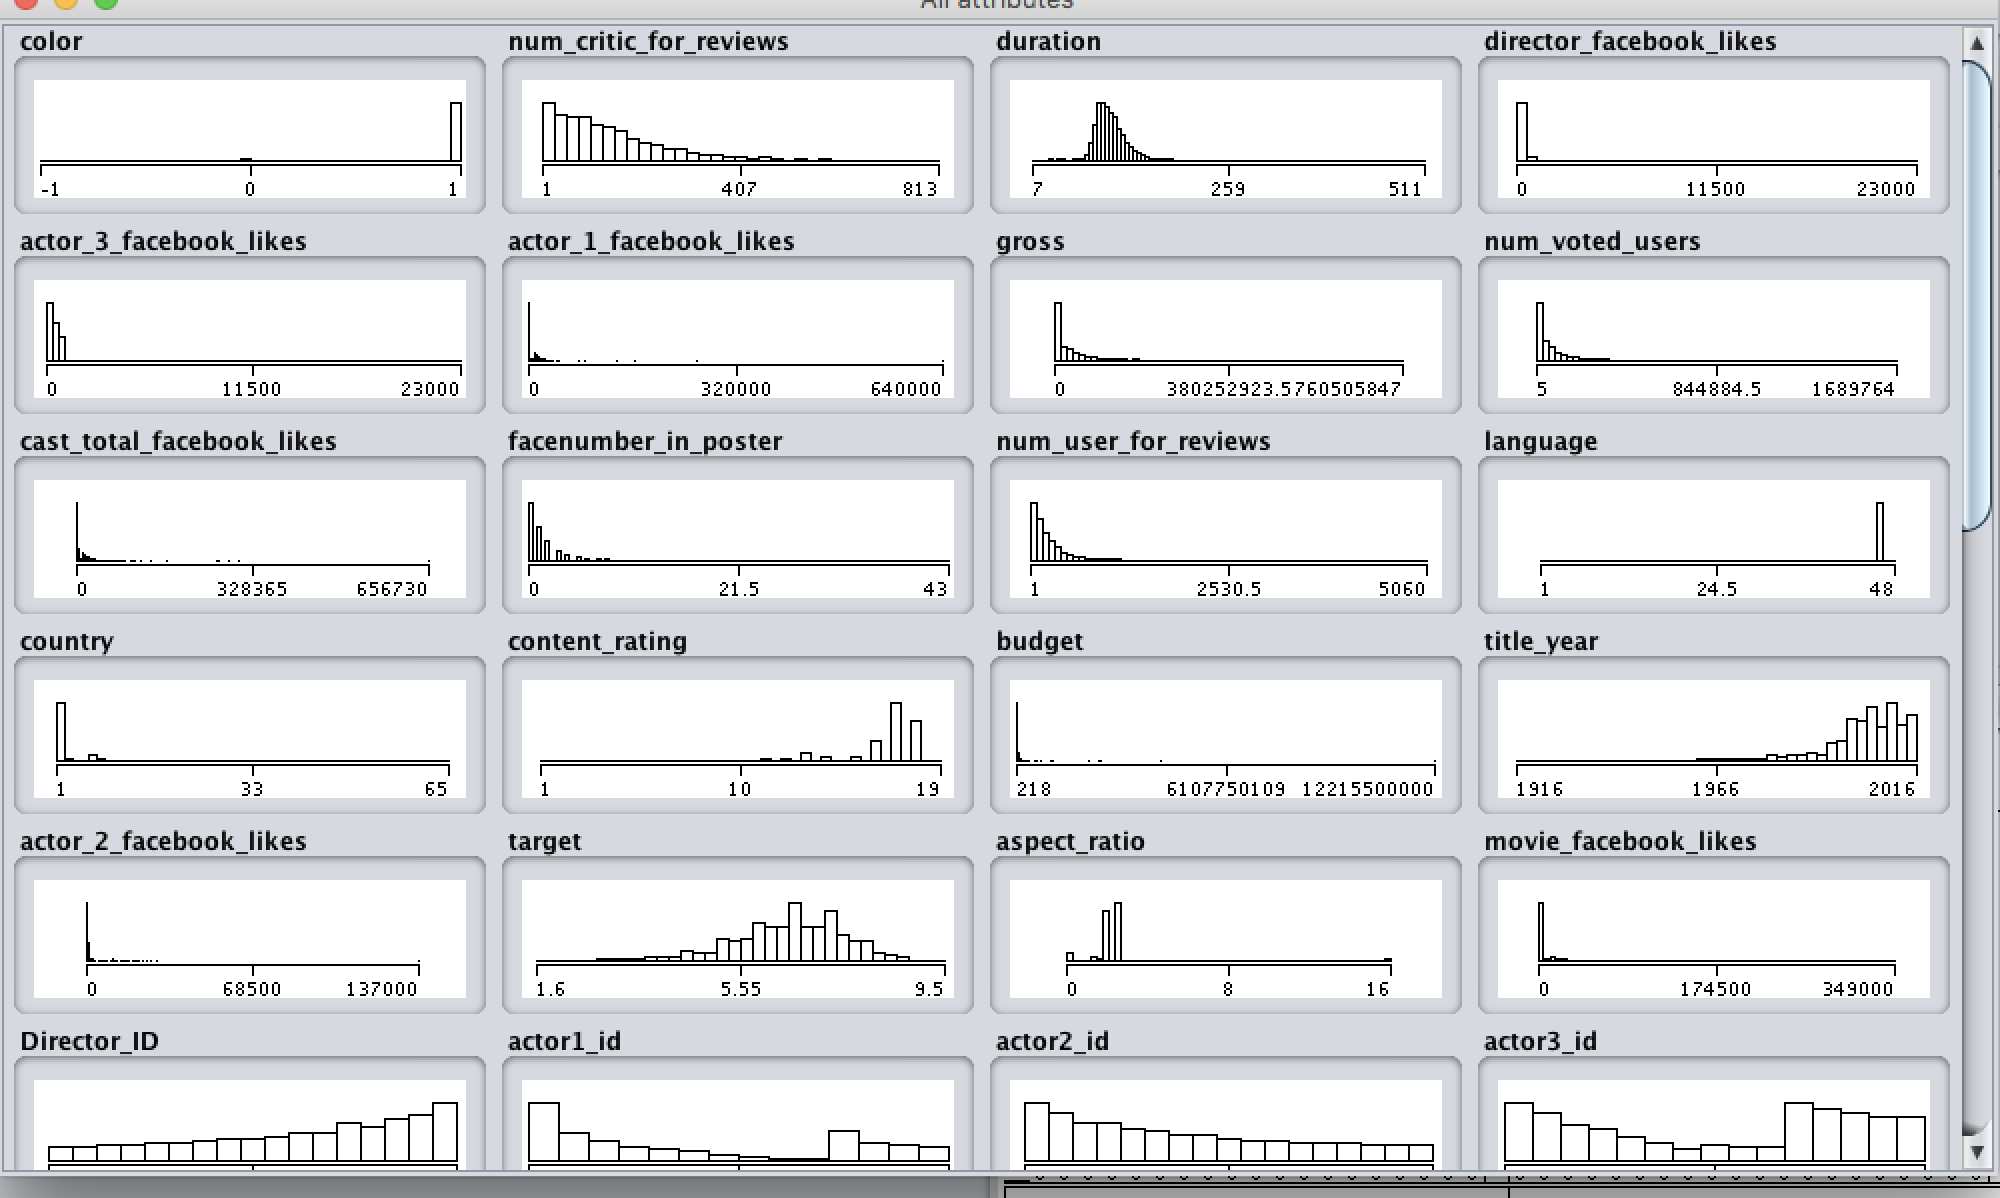
\includegraphics[height=7cm]{imagens/wekadistribuition.png}
\caption{Distribuição dos valores dos dados}
\label{distribuicao}
\end{figure}

Com o WEKA, é possível criar modelos de classificação e de clusterização. Nesse caso, foi usado o de classificação (figura \ref{classificationinterface}).

\begin{figure}[H]
\centering
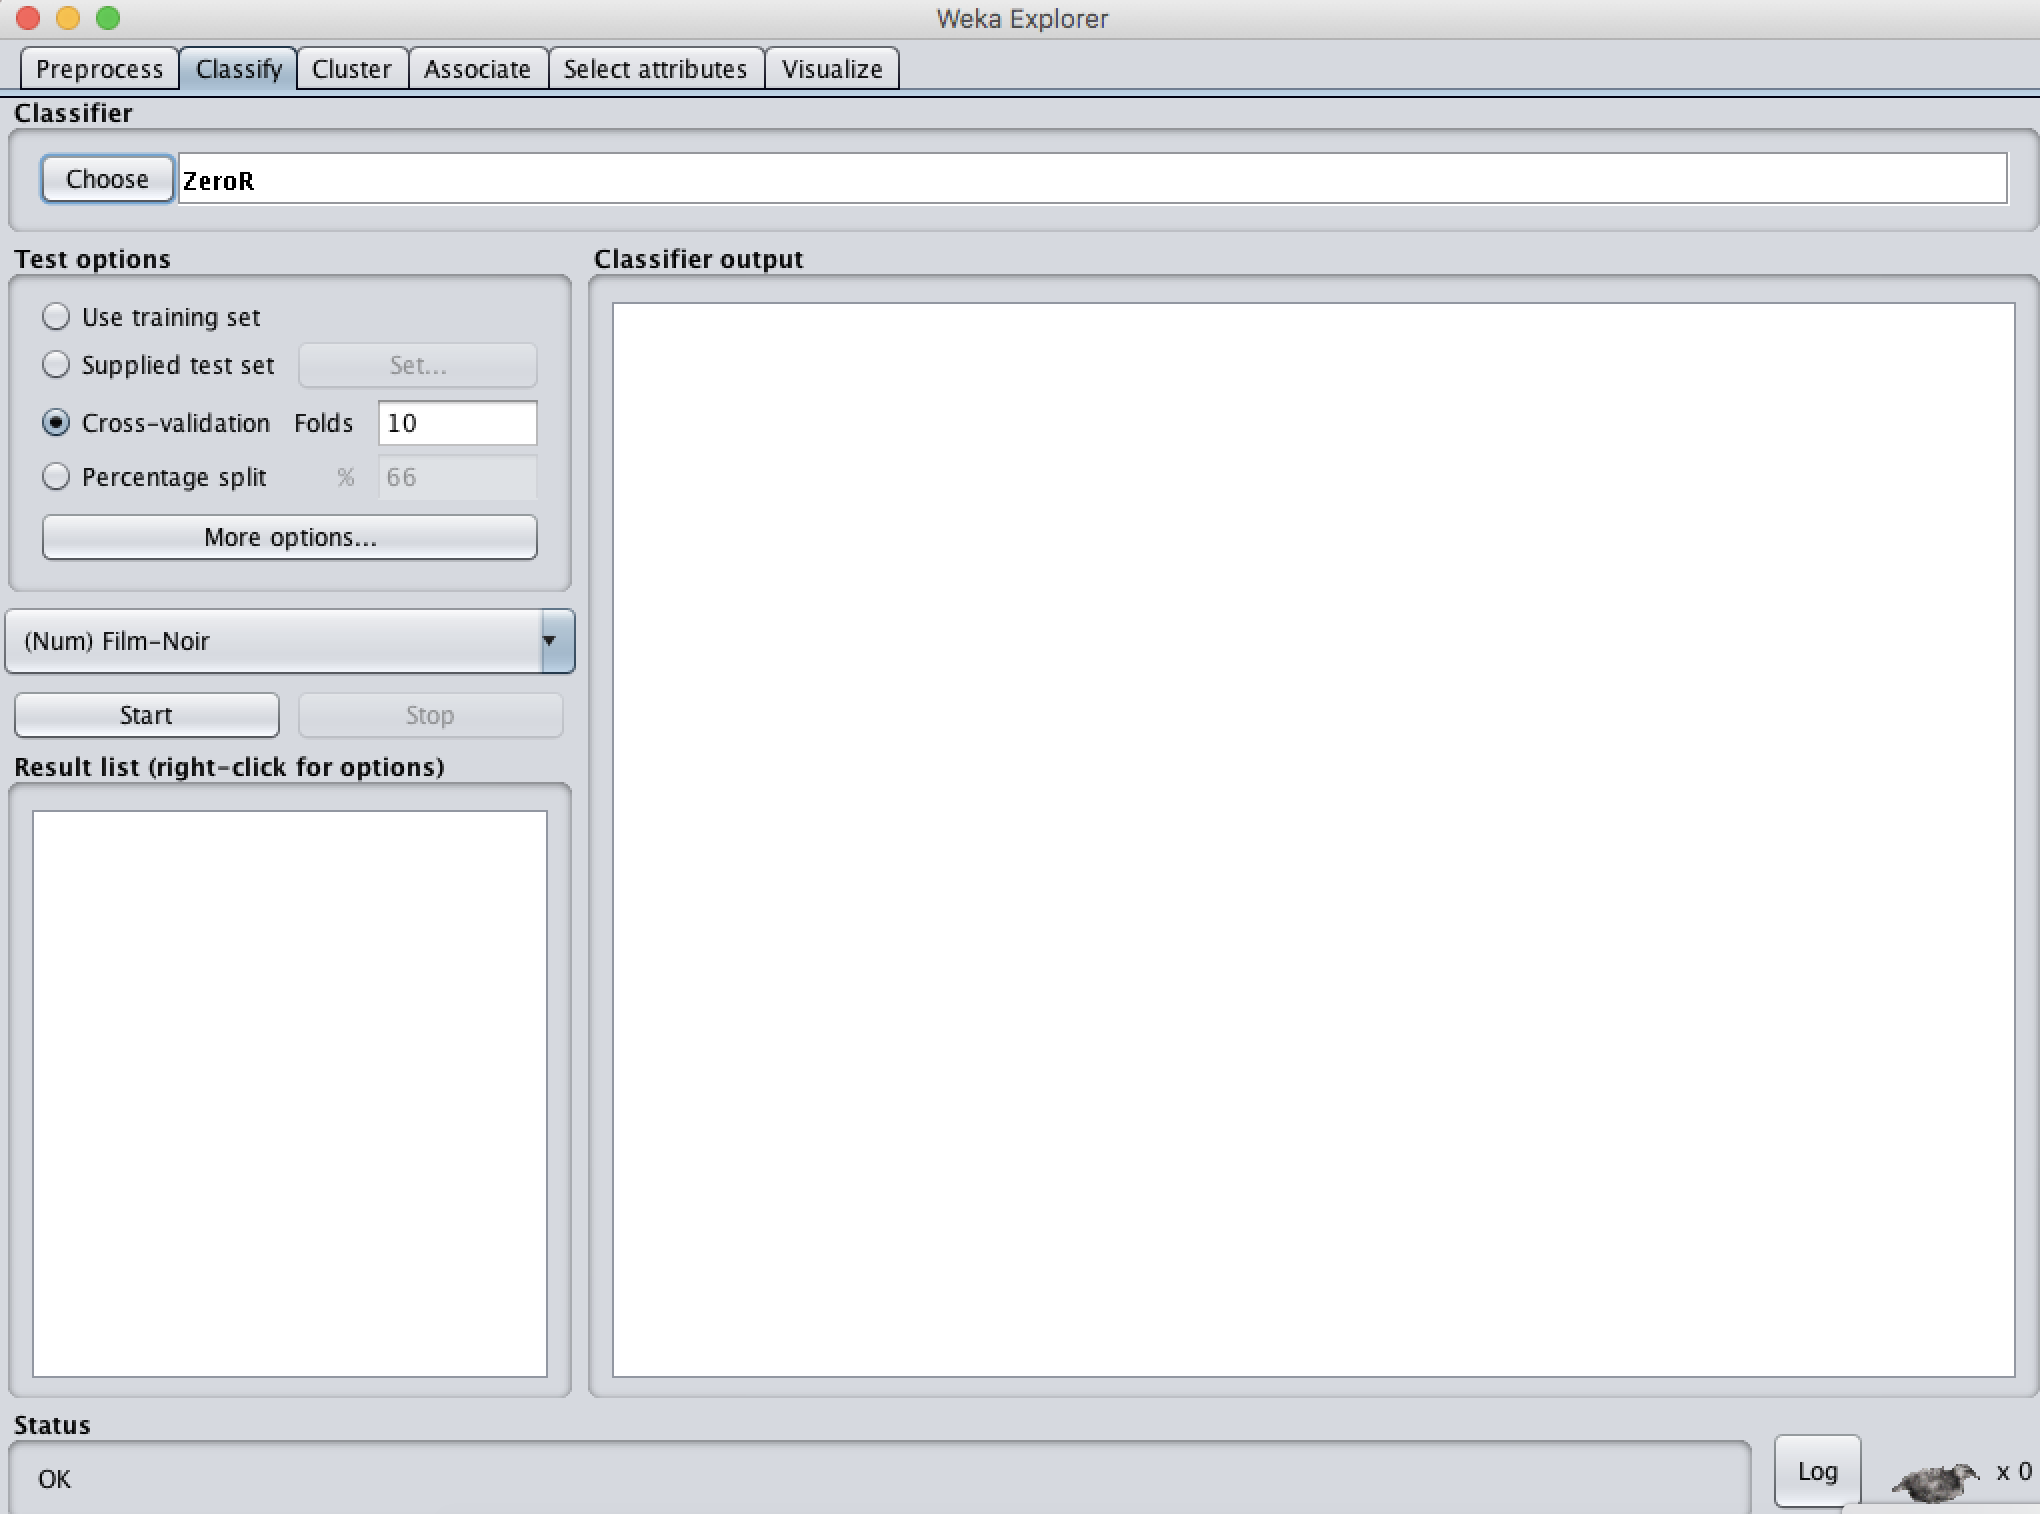
\includegraphics[height=7cm]{imagens/weka.png}
\caption{Interface de classificação}
\label{classificationinterface}
\end{figure}

Ao selecionar um algoritmo de classificação, o campo da direita irá mostrar um \textit{log} do modelo, junto com o resultado encontrado.
\begin{figure}[H]
\centering
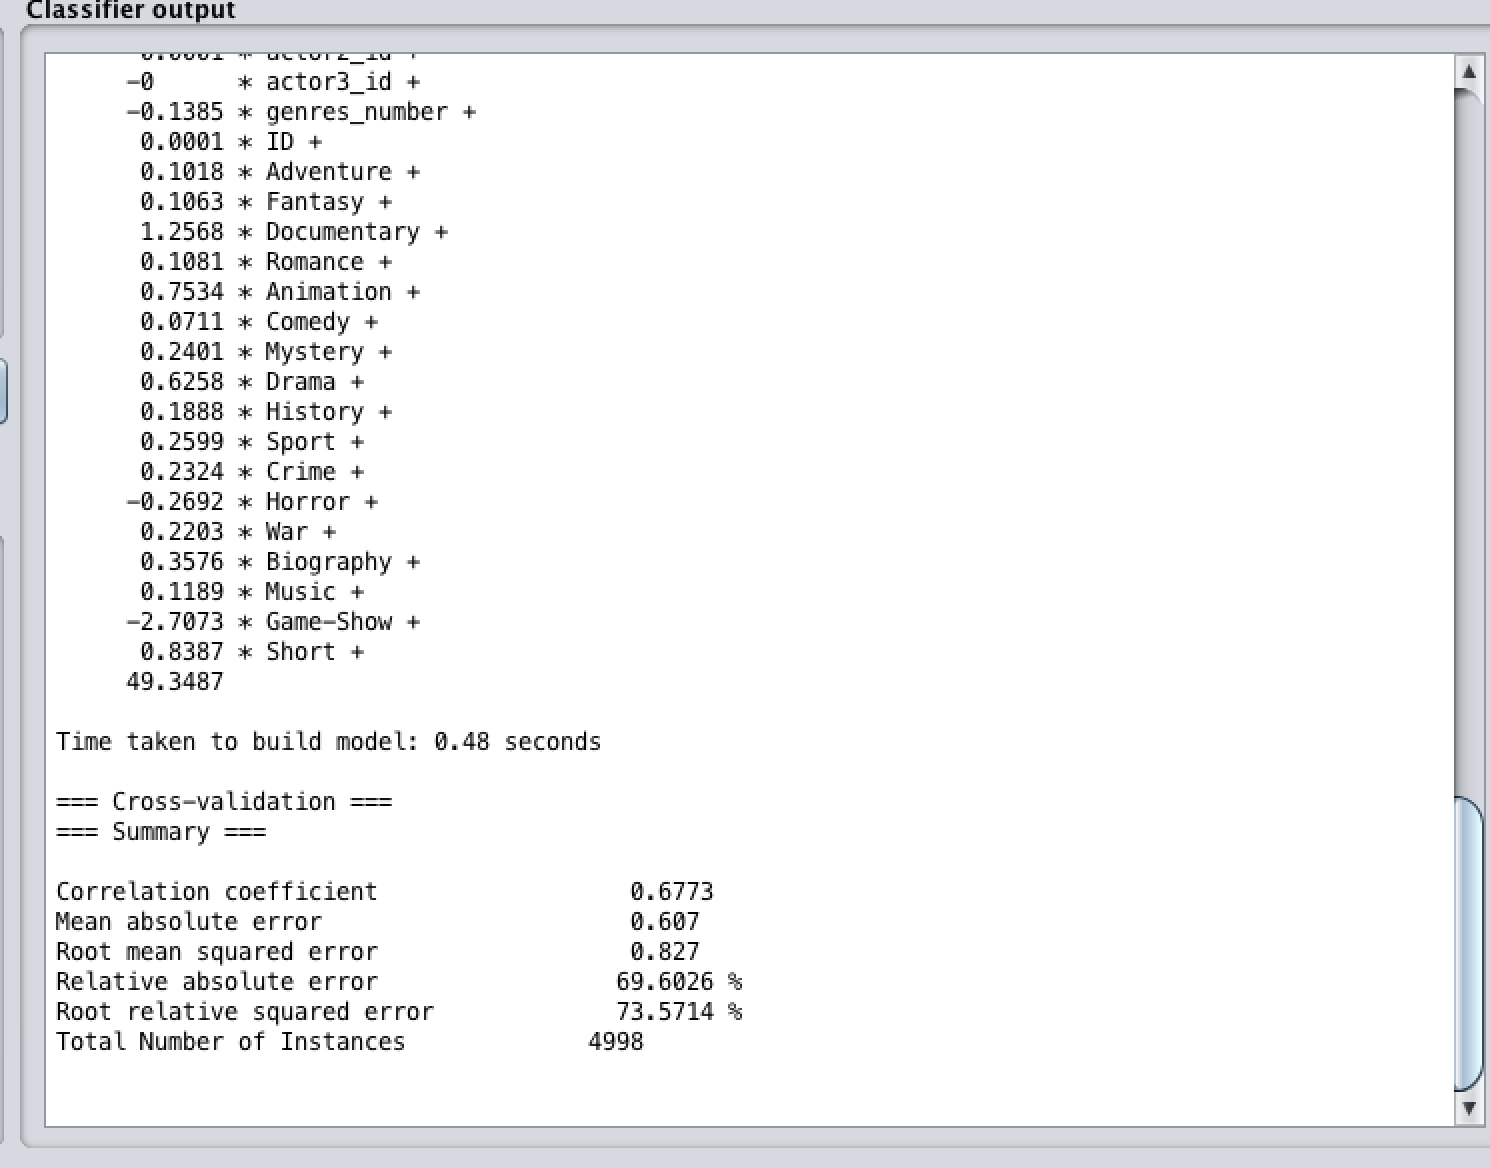
\includegraphics[height=7cm]{imagens/wekauotput.png}
\caption{Dados carregados}
\label{figura23}
\end{figure}